
并发程序的开发通常挺难的。有几个因素会使它变得更加困难:例如,编写同时需要正确和高效(换句话说,所有这些都需要)的并发程序要困难得多。对于具有许多互斥对象或无锁程序的复杂程序会更加困难。

正如在上一节的结语中所说的,管理这种复杂性的唯一方法就是对其进行封装,放入定义良好的代码或模块中。只要接口和需求是明确的,这些模块的使用者就不需要知道实现是无锁的还是基于锁的。它确实会影响性能,所以在优化之前,模块对于特定的需求可能不够用,但我们会根据需要进行优化,而且这些优化仅限于特定的模块。

在本章中,我们将重点讨论为并发编程实现数据结构的模块。为什么是数据结构而不是算法?首先,有很多关于并发算法的文献。其次,大多数开发者在处理算法上都有更宽纵的时间:分析代码,相应函数花费了过多的时间,再找到了一种不同的方法来实现算法,并在性能图表上移动到下一个高度。然后,最终会得到一个程序,其中没有一个单独的计算需要花费大量的时间,但您仍然会有它没有达到它应该达到的速度的感觉。我们以前说过,但这需要重复:当没有热代码时,就可能有热数据。

数据结构在并发程序中扮演着更重要的角色,因为它们决定了如何保证算法的可依赖性,以及限制是什么。哪些并发操作可以在相同的数据上安全执行?不同线程看到的数据视图是否一致?如果不知道这些问题的答案,我们就无法编写代码,而答案是由对数据结构的选择而决定的。

与此同时,设计决策,比如接口和模块边界的选择,会对我们编写并发程序时的选择产生重大影响,并发不能作为事后的想法添加到设计中。在设计时,从一开始就必须考虑到并发性,特别是数据的组织。

我们通过定义一些基本的术语和概念开始探索并发数据结构。

\subsubsubsection{6.4.1\hspace{0.2cm}并发数据结构的基础}

使用多线程的并发程序需要线程安全的数据结构。但是什么是线程安全,怎么使数据结构是线程安全的?乍一看,这似乎很简单:如果一个数据结构可以被多个线程同时使用,而没有任何数据竞争(在线程之间共享),那么它就是线程安全的。

然而,这个定义过于简单:

\begin{itemize}
\item 将标准定的很高——例如,没有一个STL容器是线程安全的。
\item 具有非常高的性能开销。
\item 这通常是不必要的,开销也是如此。
\item 除此之外,在许多情况下是完全无用的。
\end{itemize}

我们将逐一解决这些问题。为什么线程安全的数据结构即使在多线程程序中也是不必要的?一种微小的可能性是,用于程序的单线程部分。我们努力最小化这些部分,因为它们对总体运行时的有害影响(还记得Amdahl定律吗?),但是大多数程序都有一些需要单线程处理的事情,我们使这些代码更快的方法是只针对必要的开销。更常见的不需要线程安全的情况是,一个对象仅由一个线程使用,即使是在多线程程序中。这是非常常见的,也是非常可取的:正如我们多次说过的,共享数据是并发程序中效率低下的主要原因,因此我们试图在每个线程上只使用本地对象和数据,独立地完成尽可能多的工作。

但是,我们能确定在多线程程序中使用一个类或一个数据结构是安全的吗?即使每个对象永远不会在线程之间共享。这还真不一定:仅仅因为我们在接口层没有看到任何共享,并不意味着在实现层没有共享。多个对象可以在内部共享相同的数据:静态成员和内存分配器只是其中的一些可能性(我们倾向于认为所有需要内存的对象都通过调用\texttt{malloc()}获得,并且\texttt{malloc()}是线程安全的,而且类也可以实现自己的分配器)。

另一方面,只要没有线程修改对象,在多线程代码中使用许多数据结构是安全的。虽然这似乎是显而易见的,但我们必须再次考虑实现:接口可以是只读的,但实现仍然是可以修改对象。如果你认为这是一种奇异的可能性,请考虑标准的C++共享指针\texttt{std::shared\_ptr}:当复制一个共享指针时,复制的对象不会被修改,至少不会可见(它是通过\texttt{const}引用传递给新指针的构造函数的)。与此同时,知道对象中的引用计数必须增加,这意味着复制的对象已经改变(在此场景中,共享指针是线程安全的,但这不是偶然发生的,也不是免费的,同样也有性能成本)。

我们需要一个更细致的线程安全定义。不幸的是,对于这个普遍的概念,没有通用的标准,但是有几个流行的版本。线程安全的最高级别通常称为\textbf{强线程安全保证},意思是:提供这种保证的对象可以被多个线程并发使用,而不会引起数据竞争或其他未定义的行为(特别是,任何类不变量都会保留)。下一级称为\textbf{弱线程安全保证},只要所有线程都限制为只读访问(调用类的\texttt{const}成员函数),提供这种对象就可以使用多个线程同时访问。其次,任何对对象具有独占访问权的线程都可以对对象执行其他的操作(无论其他线程在同一时间做什么)。不提供任何此类保证的对象,根本不能在多线程程序中使用:即使对象本身不共享,其实现内部的某些内容也很容易被其他线程修改。

本书中,我们将使用强弱线程安全的语言保证。提供强担保的类有时简单地称为\textbf{线程安全}。如果该类只提供弱保证,则称为\textbf{线程兼容}。大多数STL容器都提供了这样的保证:如果容器是一个线程的局部对象,可以以任何有效的方式使用它,但如果容器对象是共享的,只能调用\texttt{const}成员函数。最后,根本不提供任何保证的类被称为\textbf{线程敌对},并且不能使用在多线程程序中。

实践中,我们经常遇到强保证和弱保证的组合:接口的一个子集提供强保证,但其余部分只提供弱保证。

那么,为什么不尝试在设计每个对象时都有强线程安全保证呢?我们已经提到的第一个原因是:会有性能开销,保证通常是不必要的,因为对象不是在线程之间共享的,编写高效程序的关键是不做无用的工作。更有趣的反对意见是我们前面提到的:即使在以需要线程安全的方式共享对象,强线程安全保证可能是无用的。假如需要开发一款玩家招募军队并进行战斗的游戏。军队中所有单位的名称都存储在一个容器中,比如一个字符串列表。另一个容器存储每个单元的当前强度。在战役中,单位总是会被杀死或招募,游戏引擎是多线程的,需要有效地管理庞大的军队。虽然STL容器只提供弱线程安全保证,但假设我们有一个强线程安全容器库。很容易看出这是不够的:添加一个单元需要将它的名称插入到一个容器中,并将它的初始强度插入到另一个容器中,这两个操作本身都是线程安全的。一个线程创建一个新单元并将其插入到第一个容器中。在这个线程还可以添加它的强度值之前,另一个线程看到这个新单位并需要查找它的强度,但是在第二个容器中还没有任何东西。问题在于线程安全保证是在错误的层面上提供的:从应用程序的角度来看,创建一个新单元是一个事务,所有游戏引擎线程都应该能够在添加单元之前或之后查看数据库,但不能在中间状态。例如,可以通过使用互斥锁来实现:它会在单元添加前锁定,只有在两个容器都新之后才会解锁。然而,在这个场景中,我们不关心单个容器提供的线程安全保证,只要这些对象的所有访问都由互斥锁保护。显然,我们需要的是一个单元数据库,它本身提供所需的线程安全保证,例如:通过使用互斥对象。这个数据库可能在内部使用几个容器对象,数据库的实现可能需要或不需要这些容器的任何线程安全保证,但这对数据库的使用者应该是不可见的(拥有线程安全的容器可能会使实现更容易,也可能不会)。

这让我们得出一个非常重要的结论:线程安全始于设计阶段。必须明智地选择程序使用的数据结构和接口,以便它们表示适当的抽象级别,以及发生线程交互级别上的正确事务。

考虑到这一点,本章的其余部分应该从两个方面来看:一方面,将展示如何设计和实现一些基本的线程安全的数据结构,这些数据结构可以用作在程序中需要的更复杂(和更多样化)的构建块。另一方面,还展示了构建线程安全类的基本技术,这些类可用于设计这些更复杂的数据结构。

\subsubsubsection{6.4.2\hspace{0.2cm}计数器和累加器}

最简单的线程安全对象是简单的计数器或累加器,计数器只是计算在线程上可能发生的一些事件。所有线程都可能需要修改计数器或访问当前值,因此存在竞争条件。

弱线程安全保证无法满足我们的要求,这里需要强线程安全保证。从而确保读取没有更改的值总是线程安全的。我们已经看到了实现的可用选项:某种锁、原子操作(当有原子操作时)或无锁CAS循环。

锁的性能因实现的不同而不同,通常首选自旋锁。没有立即访问计数器的线程的等待时间将非常短,因此将线程置于睡眠状态,并在稍后将其唤醒的成本没什么意思。另一方面,由于繁忙等待(轮询自旋锁)而浪费的CPU时间可以忽略不计,很可能只需要几条指令。

原子指令提供了良好的性能,但操作的选择相当有限:在C++中,可以原子地对整数进行加法,但不能做另一些事,例如:对整数进行乘法。这对于简单的计数器来说已经足够了,但是对于累加器来说可能还不够(累加操作可能有多个结果)。但是,如果有一种方法可用,那么它没有原子操作简单。

CAS循环可用于实现累加器,而不考虑我们需要使用的操作。然而,在大多数现代硬件上,性能比自旋锁的性能更好(参见图6.2),但并不是最快的选择。

当使用自旋锁访问单个变量或单个对象时,可以进一步优化自旋锁。我们可以让锁成为保护的对象的唯一引用,而不是通用标志。原子变量是指针,而不是整数,除此之外,锁定机制保持不变。因为\texttt{lock()}函数返回指向计数器的指针,所以是非标准的:

\hspace*{\fill} \\ %插入空行
\noindent
\textbf{01d\_ptrlock\_count.C}
\begin{lstlisting}[style=styleCXX]
template <typename T>
class PtrSpinlock {
	public:
	explicit PtrSpinlock(T* p) : p_(p) {}
	T* lock() {
		while (!(saved_p_ =
		p_.exchange(nullptr, std::memory_order_acquire))) {}
	}
	void unlock() {
		p_.store(saved_p_, std::memory_order_release);
	}
	private:
	std::atomic<T*> p_;
	T* saved_p_ = nullptr;
};
\end{lstlisting}

与之前的自旋锁实现相比,原子变量的含义是“颠倒”:如果原子变量\texttt{p\_}不为空,则该锁可用,否则为空。我们为自旋锁做的所有优化在这里也适用,看起来完全相同,所以我们不打算重复。另外,这个类需要一组删除复制操作(锁是不可复制的)。如果需要将锁转移,并将其释放给另一个对象,则该锁可以移动。如果锁拥有它所指向的对象,析构函数应该删除它(这结合了自旋锁和单类中唯一指针的功能)。

指针自旋锁的第一个优点是,提供了访问保护对象的唯一方式,这就不可能创建竞争条件,并在没有锁的情况下访问共享数据。第二个优点是,锁的性能通常略优于常规自旋锁,自旋锁是否优于原子操作也取决于硬件。相同的基准测试在不同的处理器上会出现非常不同的结果:

%\hspace*{\fill} \\ %插入空行
\begin{center}
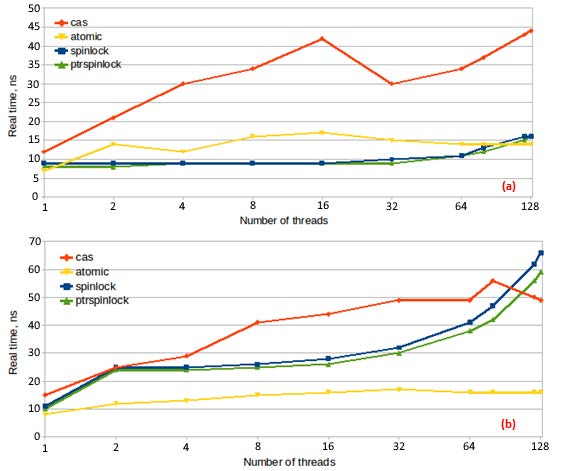
\includegraphics[width=0.9\textwidth]{content/2/chapter6/images/3.jpg}\\
图6.3 - 共享计数增量的性能:不同硬件系统(a)和(b)的常规自旋锁、指针自旋锁、无锁(比较-交换,或CAS)和无等待(原子)
\end{center}

通常,越新的处理器处理锁和繁忙等待的性能越好,而且自旋锁在最新的硬件上提供的性能也越好(图6.3中,系统\textit{b}使用的Intel X86 CPU比系统\textit{a}的CPU晚一代)。

执行一个操作所需的平均时间(或者相反的,吞吐量)是我们在大多数HPC系统中主要关注的指标。然而,这并不是用来衡量并发程序性能的唯一的指标。例如,如果程序在移动设备上运行,那么功耗可能更重要。所有线程使用的CPU总时间根据平均功耗的进行合理的调整。我们用于测量计数器增量平均实时时间的基准测试,同样也可以用来测量CPU时间:

%\hspace*{\fill} \\ %插入空行
\begin{center}
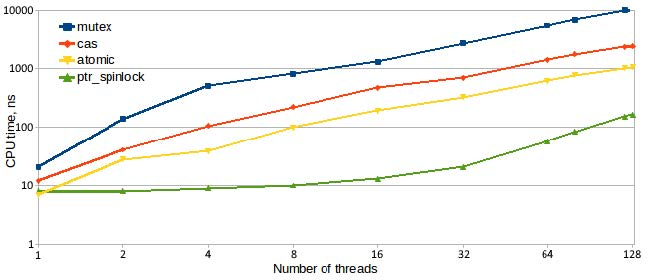
\includegraphics[width=0.9\textwidth]{content/2/chapter6/images/4.jpg}\\
图6.4 - 线程安全的计数器——不同实现使用的平均CPU时间
\end{center}

这里的坏消息是,无论采用哪种实现,多个线程同时访问共享数据的成本都会随着线程数量的增加呈指数增长,至少在有很多线程的情况下是这样的(请注意,图6.4中的y轴比例是对数的)。然而,不同的实现之间的效率差别很大,对于最高效的实现来说,在8个线程之后才会出现指数级的增长。请注意,不同硬件系统的结果也会有所不同,所以必须根据目标平台进行选择,并且只有在完成测试后才能选择。

无论选择何种实现,线程安全的累加器或计数器都不应将其公开,而应将其封装在类中。原因之一是为类的客户端提供稳定的接口,同时保留优化实现的自由度。

第二个原因更微妙,与计数器提供的保证有关。目前为止,我们关注的是计数器本身,确保所有线程都可以对其进行修改和访问,而不存在任何竞争。这是否足够使用,取决于我们如何使用计数器。如果我们想要的只是计算一些事件,而其他东西都不依赖于计数器的值,那么我们只关心值本身是否正确就好。另一方面,如果计数的是数组中的元素数量,那么我们处理的是数据依赖关系。假设有一个大型的预分配数组(或者一个容器,可以在不影响现有元素的情况下增长),所有线程都在计算要插入到这个数组中的新元素。计数器对进行计算的元素进行计数,并将值插入数组,可以由其他线程使用。换句话说,如果一个线程从计数器中读取值N,必须确保数组的前N个元素是安全读取的(这意味着没有其他线程修改它们)。但是数组本身既不是原子的,也不受锁的保护。我们可以通过锁来保护对整个数组的访问,但这可能会降低程序的性能。如果数组中已经有很多元素,任何时候只有一个线程可以读取它们,那么程序就可能是单线程的。另一方面,我们知道从多个线程读取任何常量、不可变数据都是安全的,不需要任何锁。我们只需要知道不可变数据和变化数据之间的边界在哪里,而这正是计数器应该提供的。这里的关键问题是内存可见性:需要保证在计数器的值从N-1更改为N之前,对数组前N个元素的更改对所有线程都可见。

前一章讨论内存模型时已经研究过内存可见性,那时这还是一个理论问题,但现在不是了。从上一章中,我们知道控制可见性的方法是通过限制内存序或使用内存栅栏(同一件事的两种不同的方式)。在多线程程序中,计数和索引的区别在于,索引提供了额外的保证:如果将索引从N-1增加到N的线程在增加索引之前已经完成了数组元素N的初始化,然后其他线程读取索引并获得N(或更大)的值,保证至少有N个元素完全初始化,并且可以安全地读取数组中的元素(假设没有其他线程写入这些元素)。这是一个重要的保证,不要轻易放弃:多个线程正在访问内存中的相同位置(数组元素N)而没有任何锁,其中一个线程正在写入这个位置,访问是安全的,没有数据竞争。若不能使用共享索引来确认这种保证,则需要锁定对数组的所有访问,并且在任何时候只有一个线程能够读取它。相反,我们可以使用这个原子索引类:

\hspace*{\fill} \\ %插入空行
\noindent
\textbf{02\_atomic\_index.C}
\begin{lstlisting}[style=styleCXX]
class AtomicIndex {
	std::atomic<unsigned long> c_;
	public:
	unsigned long incr() noexcept {
		return 1 + c_.fetch_add(1, std::memory_order_release);
	}
	unsigned long get() const noexcept {
		return c_.load(std::memory_order_acquire);
	}
};
\end{lstlisting}

唯一不同的索引在计数是在内存可见性保证,计数不提供:

\begin{lstlisting}[style=styleCXX]
class AtomicCount {
	std::atomic<unsigned long> c_;
	public:
	unsigned long incr() noexcept {
		return 1 + c_.fetch_add(1, std::memory_order_relaxed);
	}
	unsigned long get() const noexcept {
		return c_.load(std::memory_order_relaxed);
	}
};
\end{lstlisting}

当然,每个类的线程安全和内存可见性保证都应该有相应的文档存在。两者之间是否存在性能差异取决于硬件。而在X86 CPU上没有区别,因为是请求还是不请求,用于原子增量和原子读取的硬件指令都有“类索引”的内存栅栏存在。在ARM CPU上,自由(或无障碍)内存操作明显更快。但是,不管性能、清晰度和问题是什么,都不应该忘记:如果开发者使用一个索引类,其会显式地提供了内存序保证,但没有索引任何东西,每个读者都会想知道发生了什么,以及使用这些保证的代码中技巧和位置在哪里。通过正确的文档保证集的接口,就可以向读者表明编写这段代码的意图。

现在回到本节中的“隐藏”成就。我们学习了线程安全的计数器,但在此过程中,提出了一种算法,似乎违反了编写多线程代码的第一条规则:任何时候两个或多个线程访问相同的内存位置,访问必须带锁(或原子的)。我们没有锁定共享数组,允许在其元素中包含任意数据(所以它可能不是原子的),而且还成功了!我们用来避免数据竞争的方法是为并发设计的数据结构的基础,现在再花些时间更好地理解和概括它。

\subsubsubsection{6.4.3\hspace{0.2cm}发布协议}

我们试图解决的问题是,在数据结构设计和并发程序开发中非常常见的问题:线程正在创建新数据,程序的其余部分只能够在数据准备好时看到这些数据。创建数据的线程通常称为写线程或生产者线程,其他线程都是读取线程或消费者线程。

最简单的解决方案是使用锁,并严格遵守避免数据竞争的规则。如果多个线程(检查)必须访问相同的内存位置(检查),并且至少有一个线程在这个位置进行写操作(我们的例子中正好是一个线程——检查),那么所有线程在访问这个内存位置进行读写操作之前都必须获得锁。这种解决方案的缺点在于性能:生产者完成并且不再发生写操作之后很长一段时间,所有的消费者线程都会互相锁定,从而不能并发地读取数据。现在,只读访问根本不需要锁,但我们需要在程序中有一个保证点,这样所有的写操作都发生在这一点之前,所有的读操作都发生在这一点之后。那么可以说,所有的使用者线程都在只读环境中操作,不需要任何锁。挑战在于保证读写之间的边界,除非我们进行了某种同步,否则内存的可见性是不能保证的:仅仅因为写入器已经完成了对内存的修改,并不意味着读取器可以看到内存的最终状态。锁包括适当的内存栅栏,它们为临界区设置边界,并确保在临界区之后执行的任何操作都将看到在临界区之前或期间发生的所有内存更改。但现在我们想在没有锁的情况下,获得同样的保证。

这个问题的无锁解决方案依赖于非常特殊的协议,从而可以在生产者和消费者线程之间传递信息:

\begin{itemize}
\item 
生产者线程在内存中准备时,其他线程无法访问的数据。可以是由生产者线程分配的内存,也可以是预分配的内存。这里,生产者是唯一对该内存有有效引用的线程,而该有效引用不会与其他线程共享(可能其他线程有访问该内存的方法,但这将引起程序的错误,类似于索引数组超出边界)。因为只有一个线程访问新数据,所以不需要同步。至于其他线程,这些数据根本看不到。

\item 
所有的消费者线程都必须使用一个共享指针来访问数据,称之为\textit{根指针},这个指针最初是空的。在生产线程构造数据时,它保持为空。所以,从消费者线程的角度来看,目前没有数据。更一般地说,“指针”不需要是一个实际的指针:任何类型的句柄或引用都可以用,只要是允许访问内存位置,并且可以设置为一个预定的无效值。如果所有的新对象都是在预先分配的数组中创建的,那么“指针”实际上可以是数组的索引,无效值可以是大于或等于数组长度的任何值。

\item 
协议的关键在于,消费者访问数据的唯一方式是通过\textit{根指针},在生产者准备显示或发布数据之前,根指针保持为空。发布数据的过程非常简单:生产者必须在根指针中存储数据的正确内存位置,并且这个改变必须伴随着内存释放屏障。

\item 
协议的关键在于,消费者访问数据的唯一方式是通过\textit{根指针},在生产者准备显示或发布数据之前,\textit{根指针}保持为空。发布数据的过程非常简单:生产者必须在\textit{根指针}中存储数据的正确内存位置,并且这个改变必须伴随着内存栅栏的释放。
\end{itemize}

这个过程有时称为\textbf{发布协议},因为它允许生产者线程以一种保证没有数据竞争的方式发布信息,供其他线程使用。发布协议可以使用任何允许访问内存的句柄来实现,只要这个句柄可以进行原子性修改。当然,指针是最常用的句柄,后面是数组下标。

发布的数据可以是简单的,也可以是复杂的,这都无所谓。它甚至不必是单个对象或单个内存位置:\textit{根指针}所指向的对象本身可以包含指向多个数据的指针。发布协议的关键点为:

\begin{itemize}
\item
所有消费者都通过\textit{根指针}访问一组特定的数据。访问数据的唯一方法是读取\textit{根指针}的非空值。

\item
生产者可以以任何它想要的方式准备数据,这是\textit{根指针}仍然是空的:生产者可以对线程本地的数据进行引用。

\item 
当生产者想要发布数据时,会自动设置\textit{根指针}指向正确的地址,并释放栅栏。数据发布后,生产者不能改变它(其他线程也不能)。

\item 
消费者线程必须以原子的方式读取\textit{根指针},并获取栅栏。如果读取非空值,则可以通过\textit{根指针}读取可访问的数据。

\end{itemize}

当然,用于实现发布协议的原子读写不应该分散在代码中,应该实现一个发布指针类来封装这个功能。下一节中,我们将看到此类的一个简单版本。

\subsubsubsection{6.4.4\hspace{0.2cm}并发编程的智能指针}

并发(线程安全)数据结构的挑战是,如何以线程安全的方式添加、删除和更改数据。发布协议为我们提供了一种向所有线程发布新数据的方法,它通常是向任何此类数据结构添加新数据的第一步。因此,我们首先来了解如何将协议的指针封装入类。

\hspace*{\fill} \\ %插入空行
\noindent
\textbf{发布指针}

下面是一个发布指针,包含了\texttt{unique\_ptr}(或拥有指针)的功能(所以可以称它为线程安全的\texttt{unique\_ptr}):

\hspace*{\fill} \\ %插入空行
\noindent
\textbf{03\_owning\_ptr\_mbm.C}
\begin{lstlisting}[style=styleCXX]
template <typename T>
class ts_unique_ptr {
	public:
	ts_unique_ptr() = default;
	explicit ts_unique_ptr(T* p) : p_(p) {}
	ts_unique_ptr(const ts_unique_ptr&) = delete;
	ts_unique_ptr& operator=(const ts_unique_ptr&) = delete;
	~ts_unique_ptr() {
		delete p_.load(std::memory_order_relaxed);
	}
	void publish(T* p) noexcept {
		p_.store(p, std::memory_order_release);
	}
	const T* get() const noexcept {
		return p_.load(std::memory_order_acquire);
	}
	const T& operator*() const noexcept { return *this->get(); }
	ts_unique_ptr& operator=(T* p) noexcept {
		this->publish(p); return *this;
	}
	private:
	std::atomic<T*> p_ { nullptr };
};
\end{lstlisting}

当然,这是一个非常简单的设计。完整的实现应该支持一个自定义删除器,移动构造函数和赋值操作符,也许还有更多的特性,类似于\texttt{std::unique\_ptr}。顺便说一下,标准不能保证访问存储在\texttt{std::unique\_ptr}对象中的指针值是原子的,或者使用了必要的内存栅栏,所以\texttt{std::unique\_ptr}不能用来实现发布协议。

现在,应该清楚我们的线程安全\texttt{unique\_ptr}提供了什么。关键函数是\texttt{publish()}和\texttt{get()},它们实现了发布协议。注意,\texttt{publish()}方法不会删除旧数据,假设生产者线程只调用一次\texttt{publish()},并且只调用一个空指针。我们可以为此添加一个断言,在调试版本中这样做可能是一个好主意,但我们也关心性能问题。说到性能,基准测试显示,对发布指针进行单线程解引用的时间与原始指针或\texttt{std::unique\_ptr}的解引用时间相同。基准测试并不复杂:

\begin{lstlisting}[style=styleCXX]
struct A { … arbitrary object for testing … };
ts_unique_ptr<A> p(new A(…));
void BM_ptr_deref(benchmark::State& state) {
	A x;
	for (auto _ : state) {
		benchmark::DoNotOptimize(x = *p);
	}
	state.SetItemsProcessed(state.iterations());
}
BENCHMARK(BM_ptr_deref)->Threads(1)->UseRealTime();
… repeat for desired number of threads …
BENCHMARK_MAIN();
\end{lstlisting}

运行这个基准测试可以让我们了解对无锁发布指针的解引用有多快:

%\hspace*{\fill} \\ %插入空行
\begin{center}
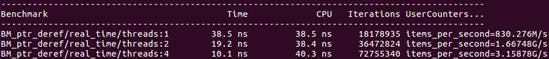
\includegraphics[width=0.9\textwidth]{content/2/chapter6/images/5.jpg}\\
图6.5 - 发布指针(消费者线程)的性能
\end{center}

结果应该与对原始指针的解引用进行比较,在多线程中也可以这样做:

%\hspace*{\fill} \\ %插入空行
\begin{center}
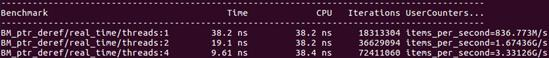
\includegraphics[width=0.9\textwidth]{content/2/chapter6/images/6.jpg}\\
图6.6 - 原始指针的性能,与图6.5进行比较
\end{center}

性能数据非常接近。我们还可以比较发布的速度,但消费者端更重要:每个对象只发布一次,然后进行多次访问。

了解发布指针不做什么同样重要。首先,在指针的构造中没有线程安全问题。我们假设生产者和消费者线程共享对构造好的指针,这个指针初始化为空。谁来构造并初始化了指针?通常,在数据结构中,都有一个\textit{根指针},通过它可以访问整个数据结构,它由构造初始数据结构的线程初始化。还有一些指针,可作为某些数据元素的根,本身包含在另一个数据元素中。现在,想象一个简单的单链表,其中每个列表元素的“next”指针是下一个元素的根,而列表的头是整个列表的根。生成列表元素的线程必须将“next”指针初始化为空。然后,另一个生产者可以添加一个新元素并发布它。请注意,这偏离了数据发布后就不可变的规则。但是,这里可以这样做,因为对线程安全\texttt{unique\_ptr}的更改都是原子的。无论如何,没有线程可以在指针构造的时候进行访问非常关键(这是一个非常常见的限制,大多数构造都不是线程安全的,因为对象在它被构造之前是不存在的,所以不能保证)。

The next thing our pointer does not do is this: it does not offer any synchronization for multiple producer threads. If two threads attempt to publish their new data elements through the same pointer, the results are undefined, and there is a data race (some consumer threads will see one set of data, and others will see different data). If there is more than one producer thread that operates on a particular data structure, they must use another mechanism for synchronization.

Finally, while our pointer implements a thread-safe publishing protocol, it does nothing to safely "un-publish" and delete the data. It is an owning pointer, so when it is deleted, so is the data it points to. However, any consumer thread can access the data using the value it had acquired earlier, even after the pointer is deleted. The issues of data ownership and lifetime must be handled in some other way. Ideally, we would have a point in the program where the entire data structure or some subset of it is known to be no longer needed; no consumer thread should try to access this data or even retain any pointers to it. At that point, the root pointer and anything accessible through it can be safely deleted. Arranging for such a point in the execution is a different matter entirely; it is often controlled by the overall algorithm.

Sometimes we want a pointer that manages both the creation and the deletion of the data in a thread-safe way. In this case, we need a thread-safe shared pointer.

\hspace*{\fill} \\ %插入空行
\noindent
\textbf{原子共享指针}

If we cannot guarantee that there is a known point in the program where the data can be safely deleted, we have to keep track of how many consumer threads hold valid pointers to the data. If we want to delete this data, we have to wait until there is only one pointer to it in the entire program; then, it is safe to delete the data and the pointer itself (or at least reset it to null). This is a typical job for a shared pointer that does reference counting: it counts how many pointers to the same object are still out there in the program; the data is deleted by the last such pointer.

When talking about thread-safe shared pointers, it is vitally important to understand precisely what guarantees are required from the pointer. The C++ standard shared pointer, std::shared\_ptr, is often referred to as thread-safe. Specifically, it offers the following guarantee: if multiple threads operate on different shared pointers that all point to the same object, then the operations on the reference counter are thread safe even if two threads cause the counter to change at the same time. For example, if one thread is making a copy of its shared pointer while another thread is deleting its shared pointer and the reference count was N before these operations started, the counter will go up to N+1, then back to N (or down first, then up, depending on the actual order of execution) and in the end will have the same value N. The intermediate value could be either N+1 or N-1, but there is no data race, and the behavior is well defined, including the final state. This guarantee implies that the operations on the reference counter are atomic; indeed, the reference counter is an atomic integer and the implementation used fetch\_add() to atomically increment or decrement it.

This guarantee applies as long as no two threads share access to the same shared pointer. How to get each thread its own shared pointer is a separate issue: since all shared pointers pointing to the same object must be created from the very first such pointer, these pointers had to have been passed from one thread to another at some point in time. For simplicity, let us assume, for a moment, that the code that made copies of the shared pointer is protected by a mutex. If two threads access the same shared pointer, then all bets are off. For example, if one thread is trying to copy the shared pointer while another thread is resetting it at the same time, the results are undefined. In particular, the standard shared pointer cannot be used to implement the publishing protocol. However, once the copies of the shared pointer have been distributed to all threads (possibly under lock), the shared ownership is maintained, and the deletion of the object is handled in a thread-safe manner. The object will be deleted once the last shared pointer that points to it is deleted. Note that, since we agreed that each particular shared pointer is never handled by more than one thread, this is completely safe. If, during the execution of the program, the time comes when there is only one shared pointer that owns our object, then there is also only one thread that can access this object. Other threads cannot make copies of this pointer (we don't let two threads share the same pointer object) and don't have any other way to get a pointer to the same object, so the deletion will proceed effectively single-threaded. This is all well and good, but what if we cannot guarantee that two threads won't try to access the same shared pointer? The first example of such access is our publishing protocol: the consumer threads are reading the value of the pointer while the producer thread may be changing it. We need the operations on the shared pointer itself to be atomic. In C++20, we can do just that: it lets us write std::atomic<std::shared\_ptr<T>>. Note that the early proposals featured a new class, std::atomic\_shared\_ptr<T>, instead. In the end, this is not the path that was chosen.

If you do not have a C++20-compliant compiler and the corresponding standard library or cannot use C++20 in your code, you can still do atomic operations on std::shared\_ptr, but you must do so explicitly. In order to publish the object using the pointer p\_ that is shared between all threads, the producer thread must do this:

\begin{lstlisting}[style=styleCXX]
std::shared_ptr<T> p_;
T* data = new T;
… finish initializing the data …
std::atomic_store_explicit(
	&p_, std::shared_ptr<T>(data), std::memory_order_release);
\end{lstlisting}

On the other hand, to acquire the pointer, the consumer thread must do this:

\begin{lstlisting}[style=styleCXX]
std::shared_ptr<T> p_;
const T* data = std::atomic_load_explicit(
	&p_, std::memory_order_acquire).get();
\end{lstlisting}

The major downside of this approach, compared to the C++20 atomic shared pointer, is that there is no protection against accidental non-atomic access. It is up to the programmer to remember to always use atomic functions to operate on the shared pointer.

It should be noted that, while convenient, std::shared\_ptr is not a particularly efficient pointer, and the atomic accesses make it even slower. We can compare the speed of publishing an object using the thread-safe publishing pointer from the last section versus the shared pointer with explicit atomic accesses:

%\hspace*{\fill} \\ %插入空行
\begin{center}
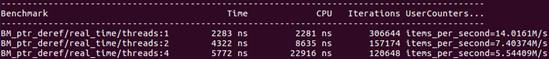
\includegraphics[width=0.9\textwidth]{content/2/chapter6/images/7.jpg}\\
Figure 6.7 – The performance of the atomic shared publishing pointer (consumer threads)
\end{center}

Again, the numbers should be compared with those from Figure 6.5: the publishing pointer is 60 times faster on one thread, and the advantage increases with the number of threads. Of course, the whole point of the shared pointer is that it provides shared resource ownership, so naturally, it takes more time to do more work. The point of the comparison is to show the cost of this shared ownership: if you can avoid it, your program will be much more efficient.

Even if you need shared ownership (and there are some concurrent data structures that are really hard to design without it), usually, you can do much better if you design your own reference-counted pointer with limited functionality and optimal implementation. One very common approach is to use intrusive reference counting. An intrusive shared pointer stores its reference count in the object it points to. When designed for a specific object, such as a list node in our particular data structure, the object is designed with the shared ownership in mind and contains a reference counter. Otherwise, we can use a wrapper class for almost any type and augment it with a reference counter:

\hspace*{\fill} \\ %插入空行
\noindent
\textbf{04\_intr\_shared\_ptr\_mbm.C}
\begin{lstlisting}[style=styleCXX]
template <typename T> struct Wrapper {
	T object;
	Wrapper(… arguments …) : object(…) {}
	~Wrapper() = default;
	Wrapper (const Wrapper&) = delete;
	Wrapper& operator=(const Wrapper&) = delete;
	std::atomic<size_t> ref_cnt_ = 0;
	void AddRef() {
		ref_cnt_.fetch_add(1, std::memory_order_acq_rel);
	}
	bool DelRef() { return
		ref_cnt_.fetch_sub(1, std::memory_order_acq_rel) == 1;
	}
};
\end{lstlisting}

When decrementing the reference count, it is important to know when it reaches 0 (or was 1 before decrementing): the shared pointer must then delete the object.

The implementation of even the simplest atomic shared pointer is quite lengthy; a very rudimentary example can be found in the sample code for this chapter. Again, this example contains only the bare minimum necessary for the pointer to correctly perform several tasks such as publishing an object and accessing the same pointer concurrently by multiple threads. The aim of the example is to make it easier to understand the essential elements of implementing such pointer (and even then, the code is several pages long).

In addition to using an intrusive reference counter, an application-specific shared pointer can forgo other features of std::shared\_ptr. For example, many applications do not require a weak pointer, but there is an overhead for supporting it even if it's never used. A minimalistic reference-counted pointer can be several times more efficient than the standard one:

%\hspace*{\fill} \\ %插入空行
\begin{center}
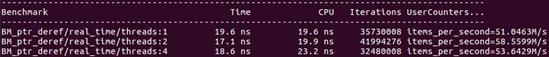
\includegraphics[width=0.9\textwidth]{content/2/chapter6/images/8.jpg}\\
Figure 6.8 – The performance of a custom atomic shared publishing pointer (consumer threads)
\end{center}

It is similarly more efficient for assignment and reassignment of the pointer, atomic exchange of two pointers, and other atomic operations on the pointer. Even this shared pointer is still much less efficient than a unique pointer, so again, if you can manage the data ownership explicitly, without reference-counting, do so.

We now have the two key building blocks of almost any data structure: we can add new data and publish it (reveal it to other threads), and we can track the ownership, even across threads (although it comes at a price).




















